% -*- latex -*-
%%%%%%%%%%%%%%%%%%%%%%%%%%%%%%%%%%%%%%%%%%%%%%%%%%%%%%%%%%%%%%%%
%%%%%%%%%%%%%%%%%%%%%%%%%%%%%%%%%%%%%%%%%%%%%%%%%%%%%%%%%%%%%%%%
%%%%
%%%% This text file is part of the source of slides for
%%%% `Introduction to High-Performance Scientific Computing'
%%%% by Victor Eijkhout, copyright 2012
%%%%
%%%%%%%%%%%%%%%%%%%%%%%%%%%%%%%%%%%%%%%%%%%%%%%%%%%%%%%%%%%%%%%%
%%%%%%%%%%%%%%%%%%%%%%%%%%%%%%%%%%%%%%%%%%%%%%%%%%%%%%%%%%%%%%%%

\Level 1 {Parallelism and implicit operations: wavefronts, approximation}

\begin{frame}{Recurrences}
    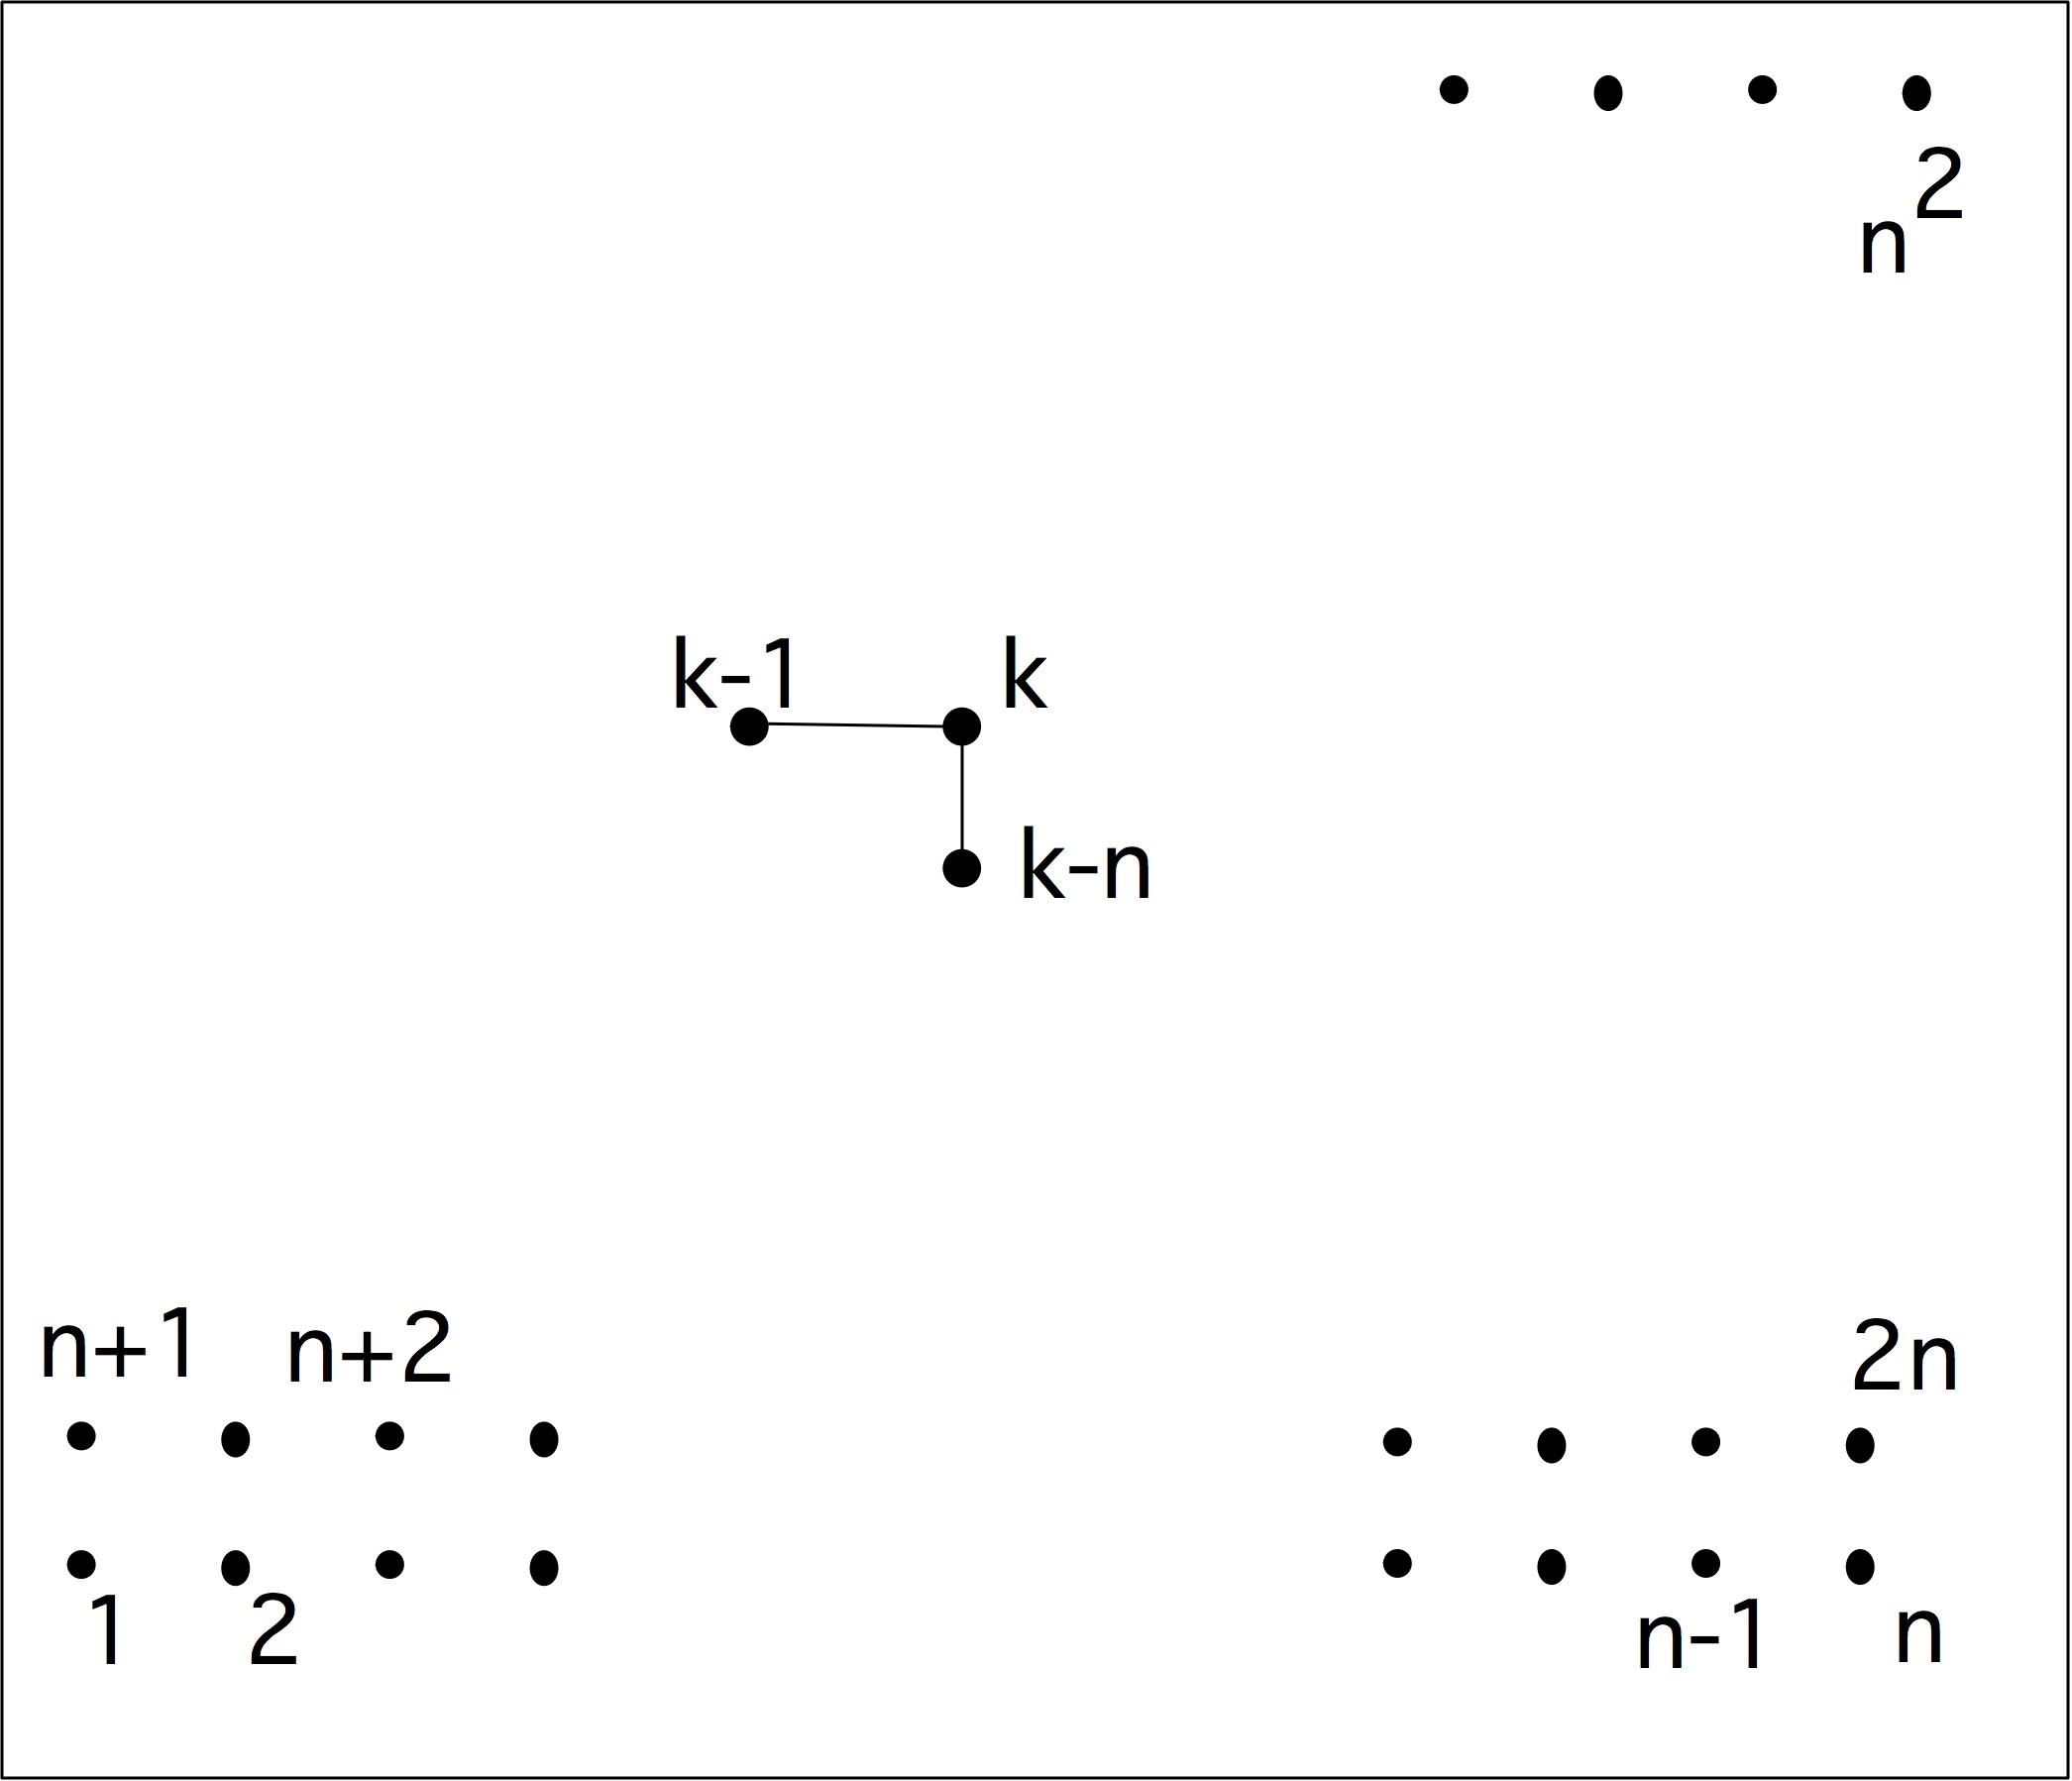
\includegraphics[scale=.09]{laplacelower}

    \[ x_{i,j} = f(x_{i-1,j},x_{i,j-1}) \]
    Intuitively: recursion length $n^2$
\end{frame}

\begin{frame}{However\ldots}
  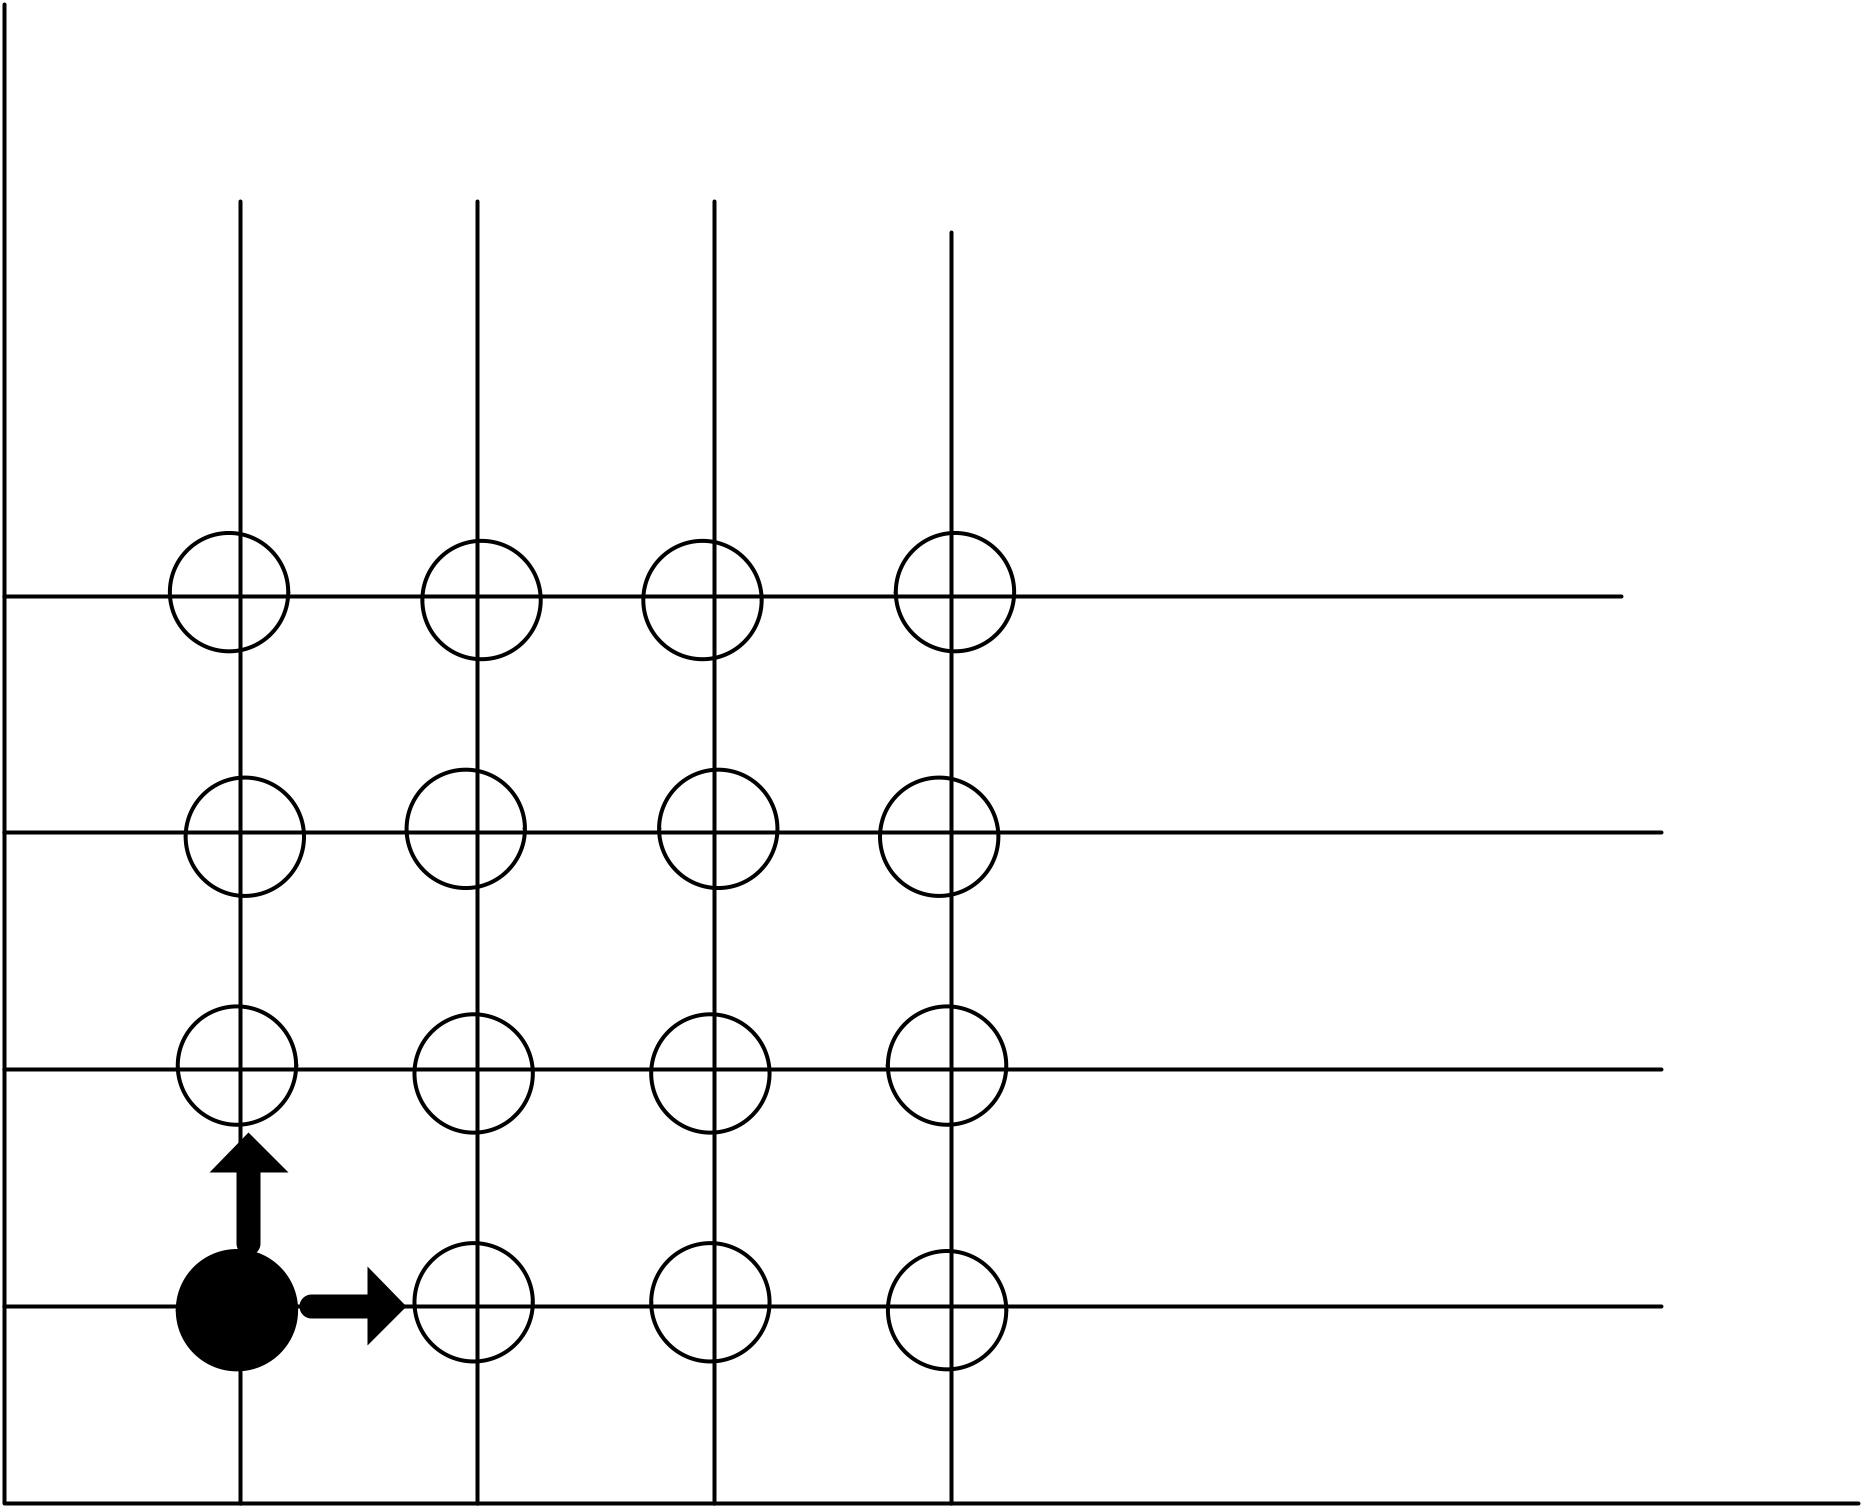
\includegraphics[scale=.1]{wavefront1}
\end{frame}

\begin{frame}
  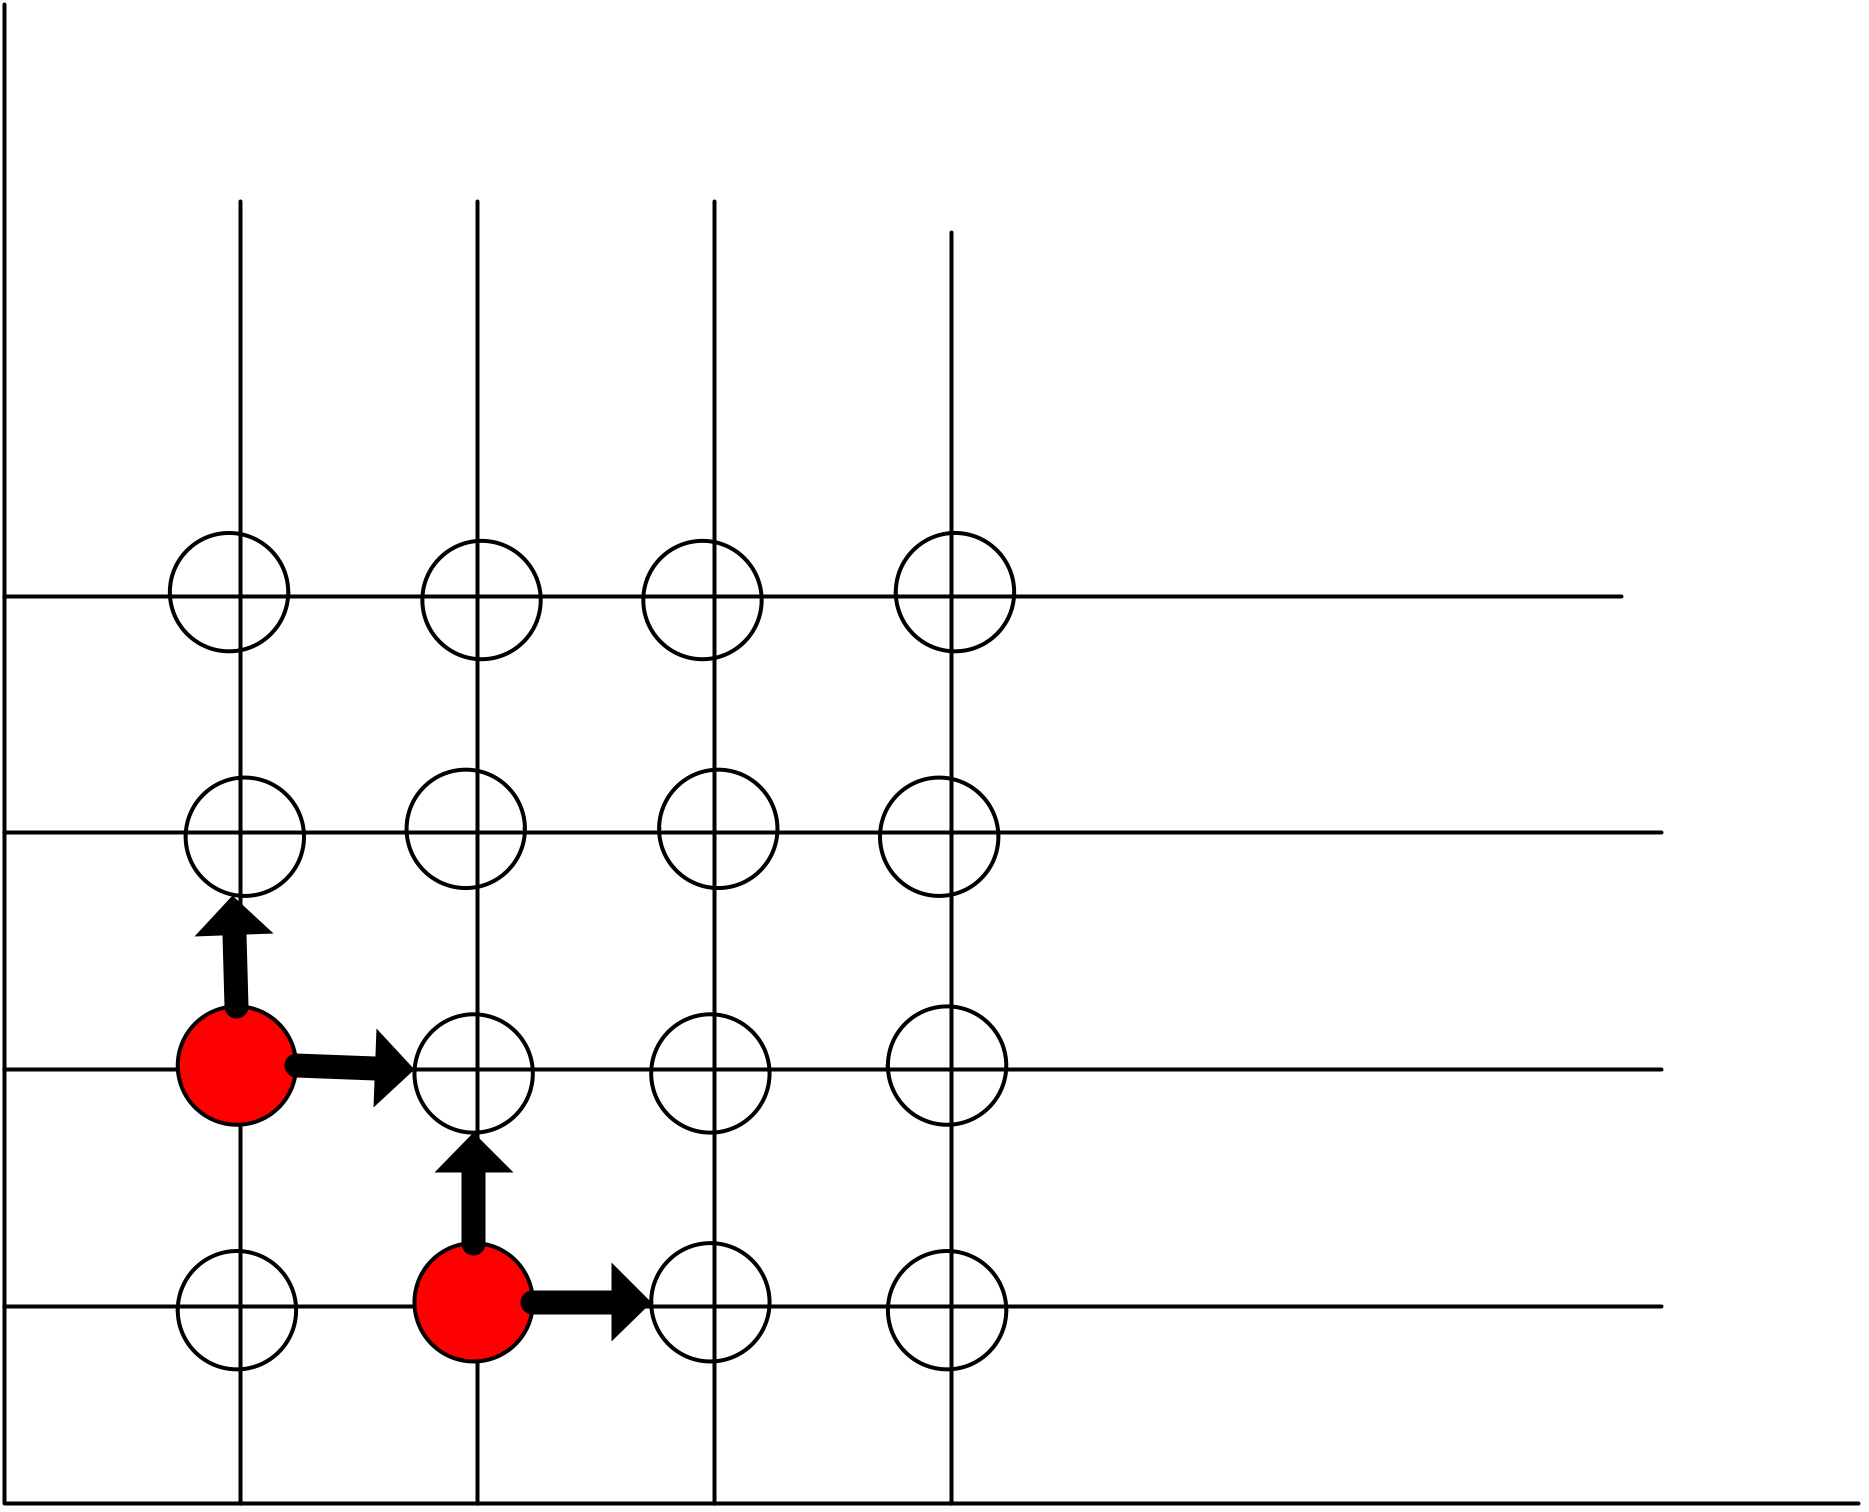
\includegraphics[scale=.1]{wavefront2}
\end{frame}

\begin{frame}
  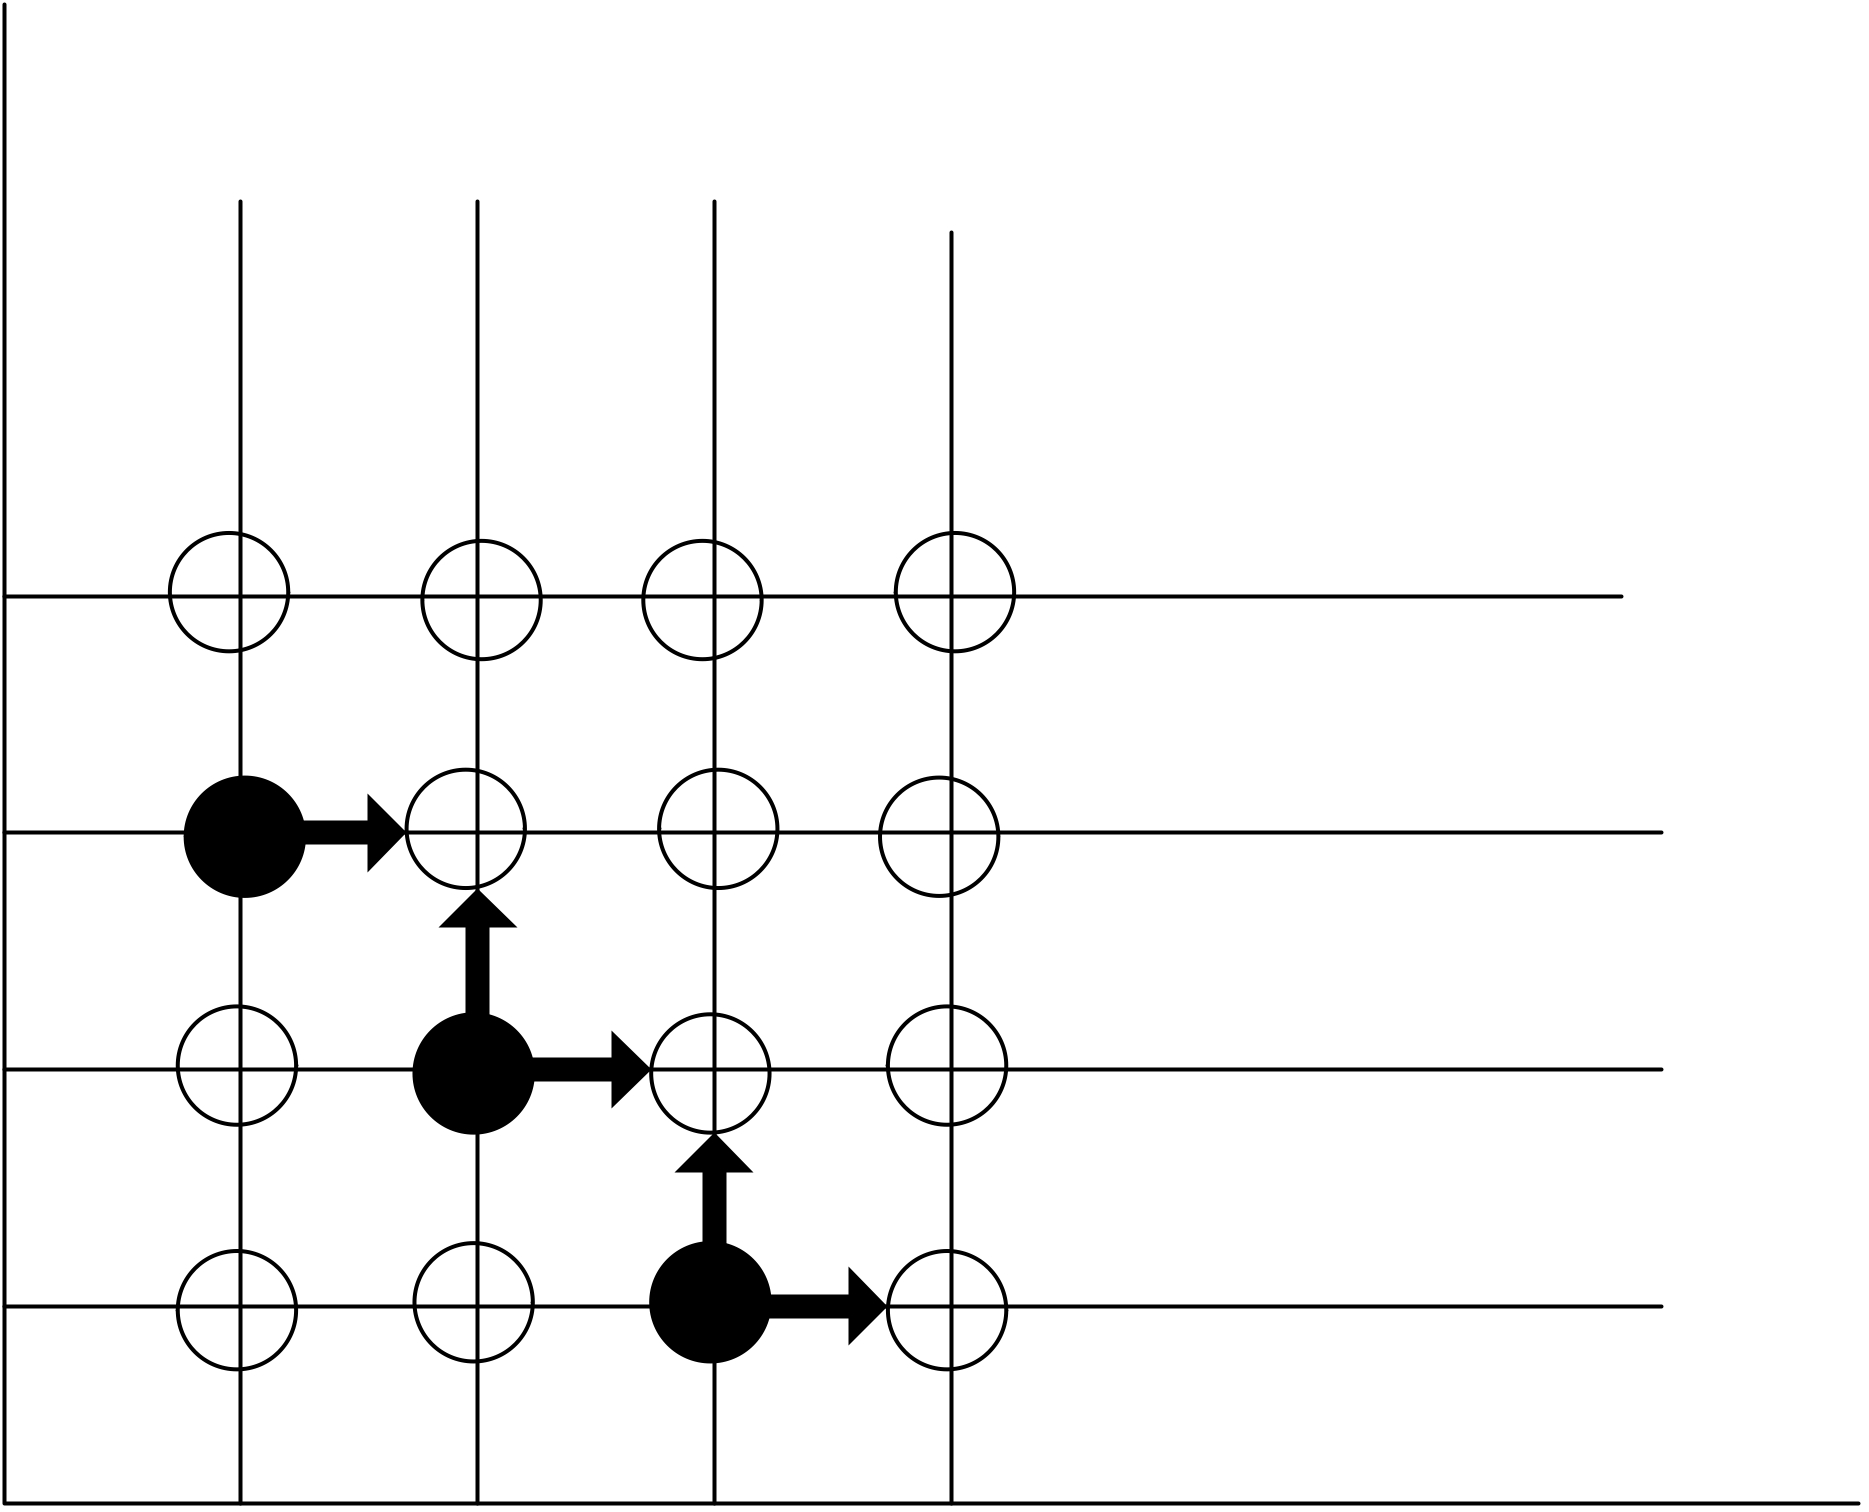
\includegraphics[scale=.1]{wavefront3}
\end{frame}

\begin{frame}{And in fact}
  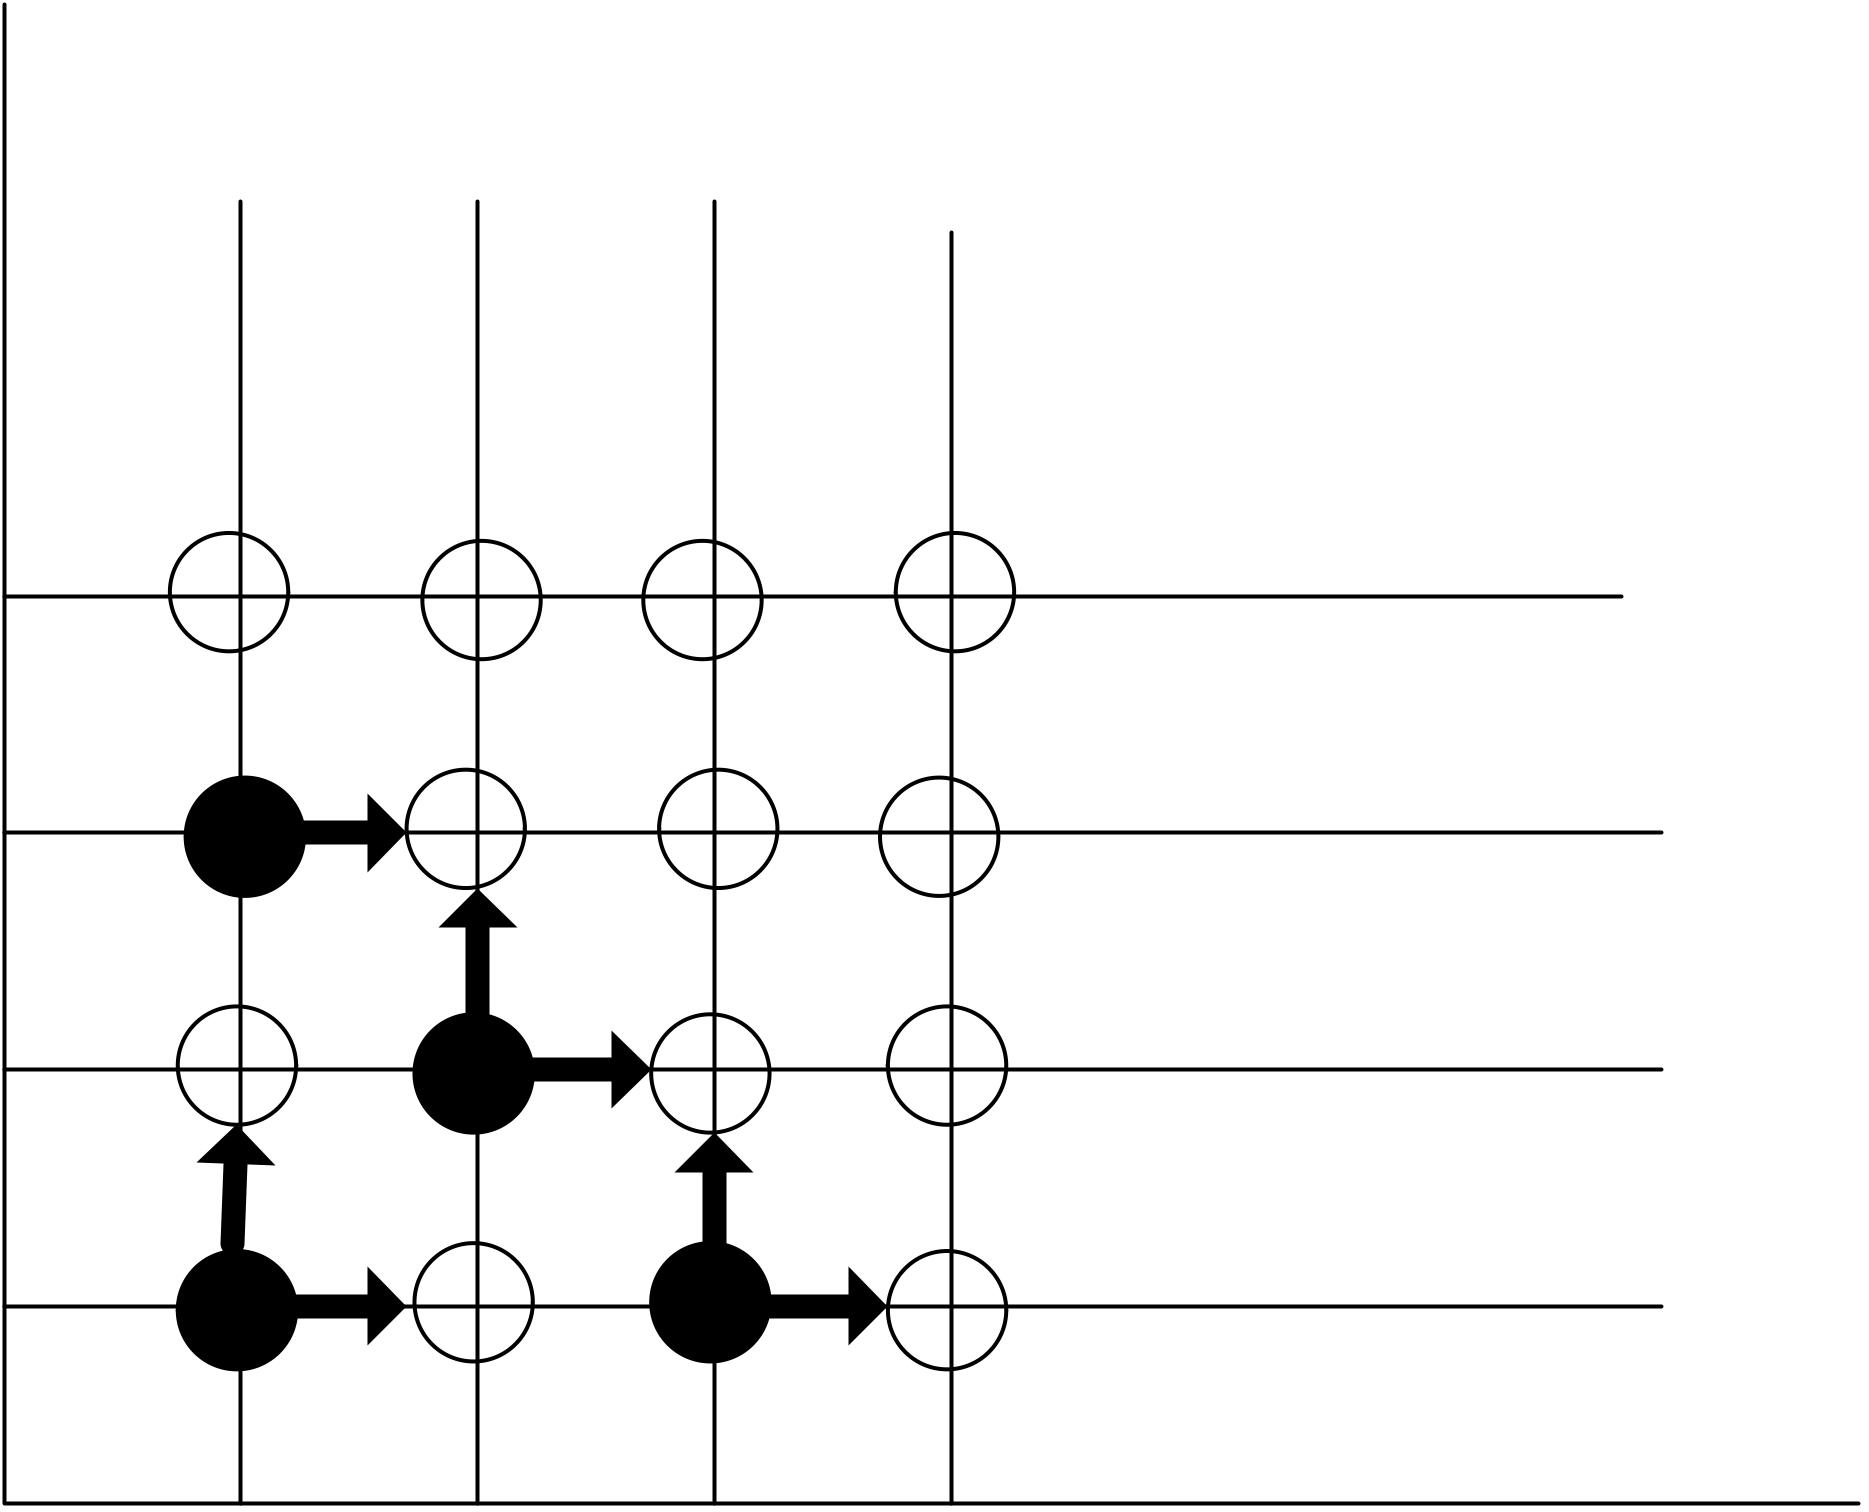
\includegraphics[scale=.1]{wavefront3b}
\end{frame}

\begin{frame}{But then too}
  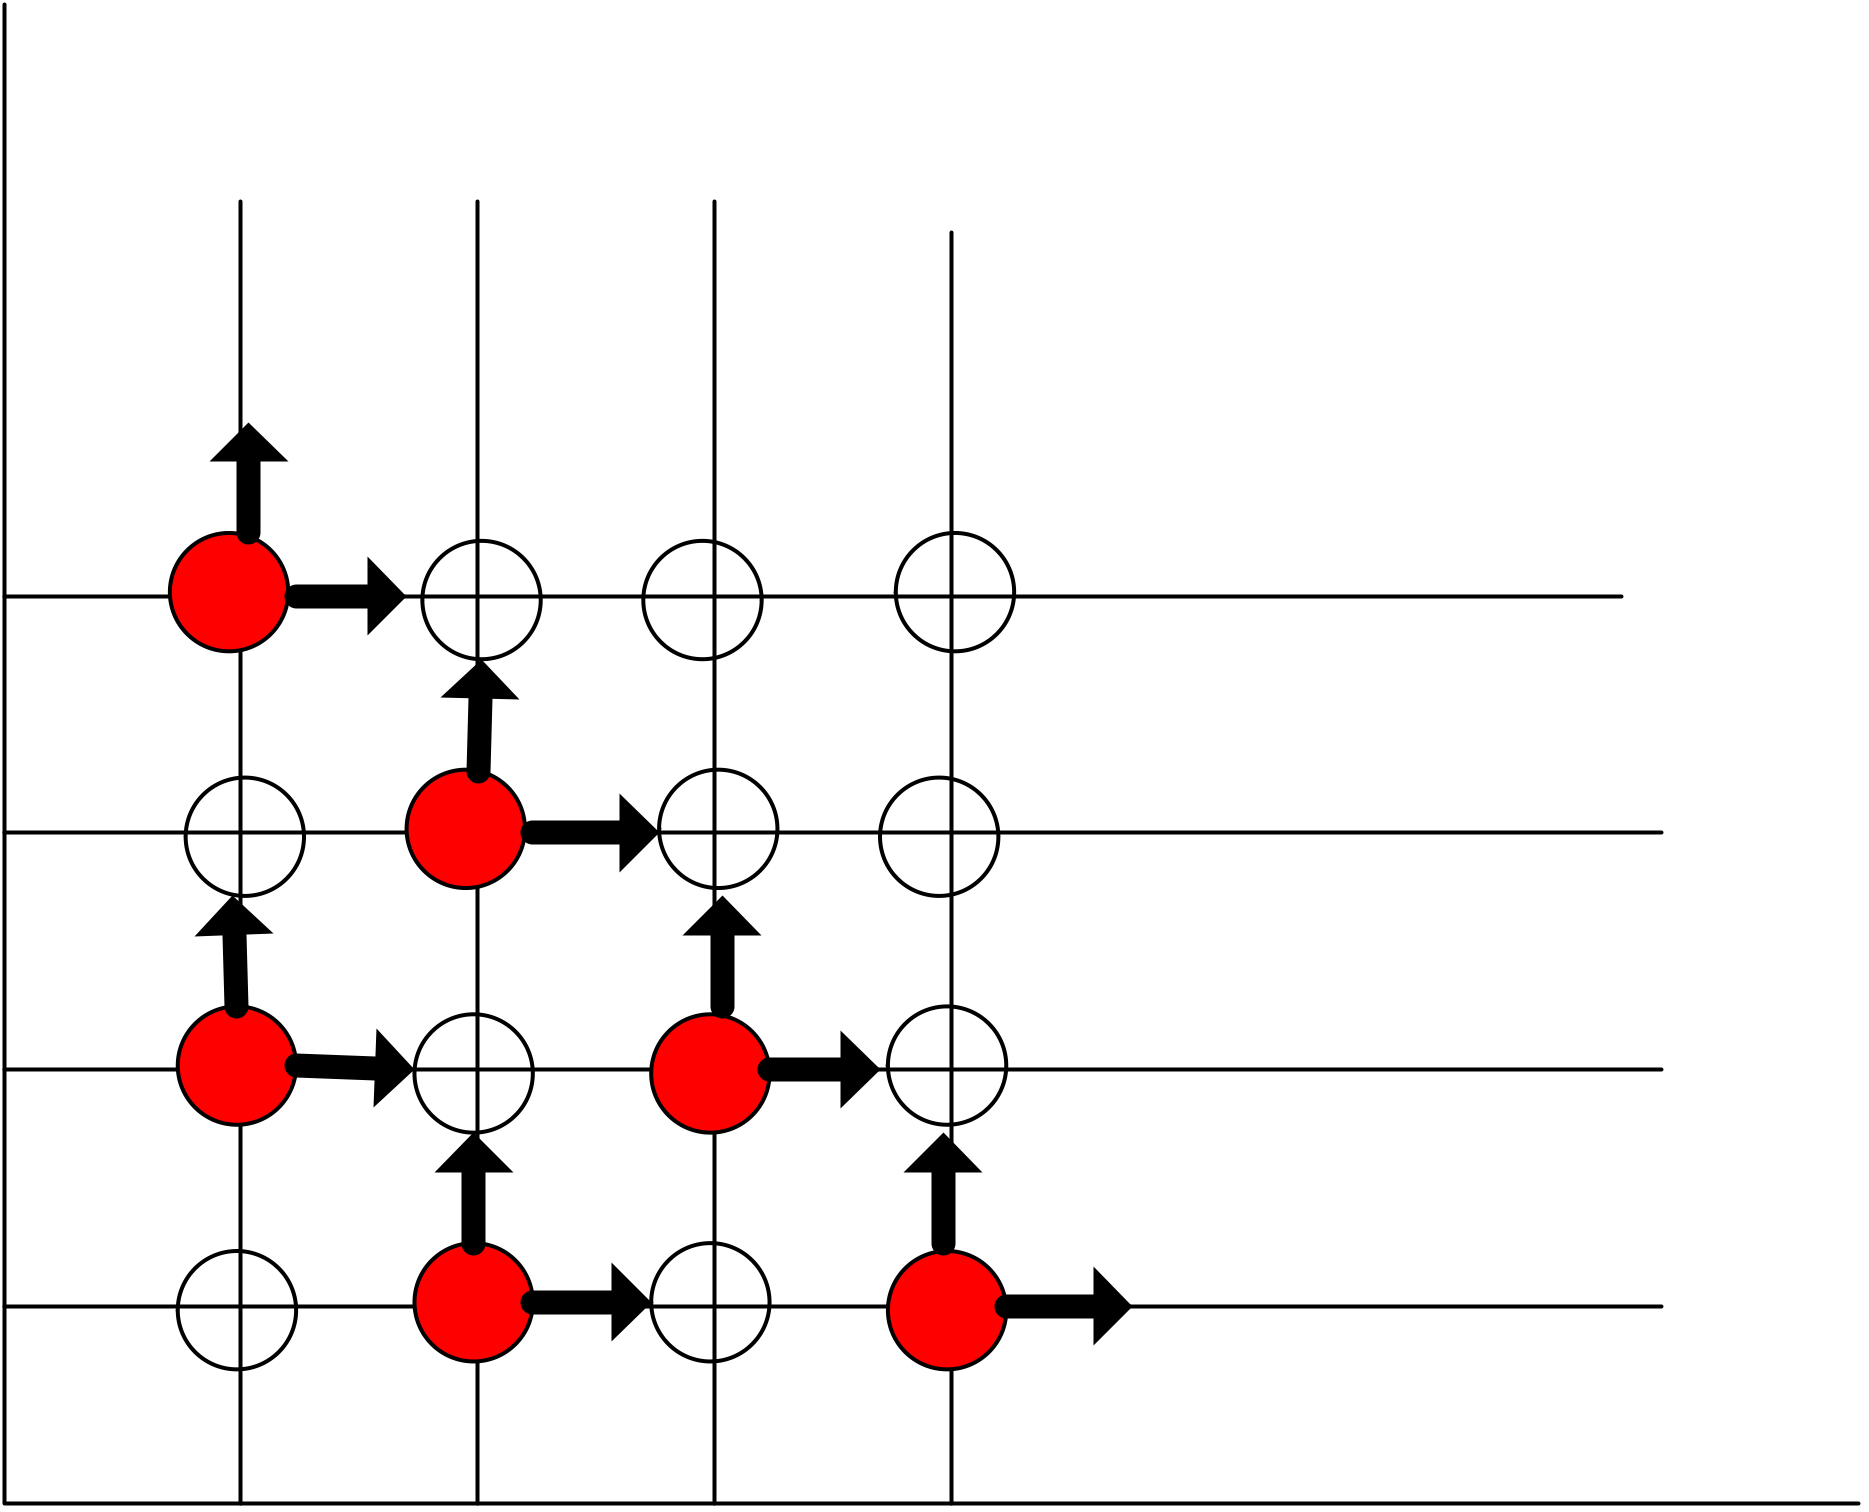
\includegraphics[scale=.1]{wavefront2b}
\end{frame}

\begin{frame}{And}
  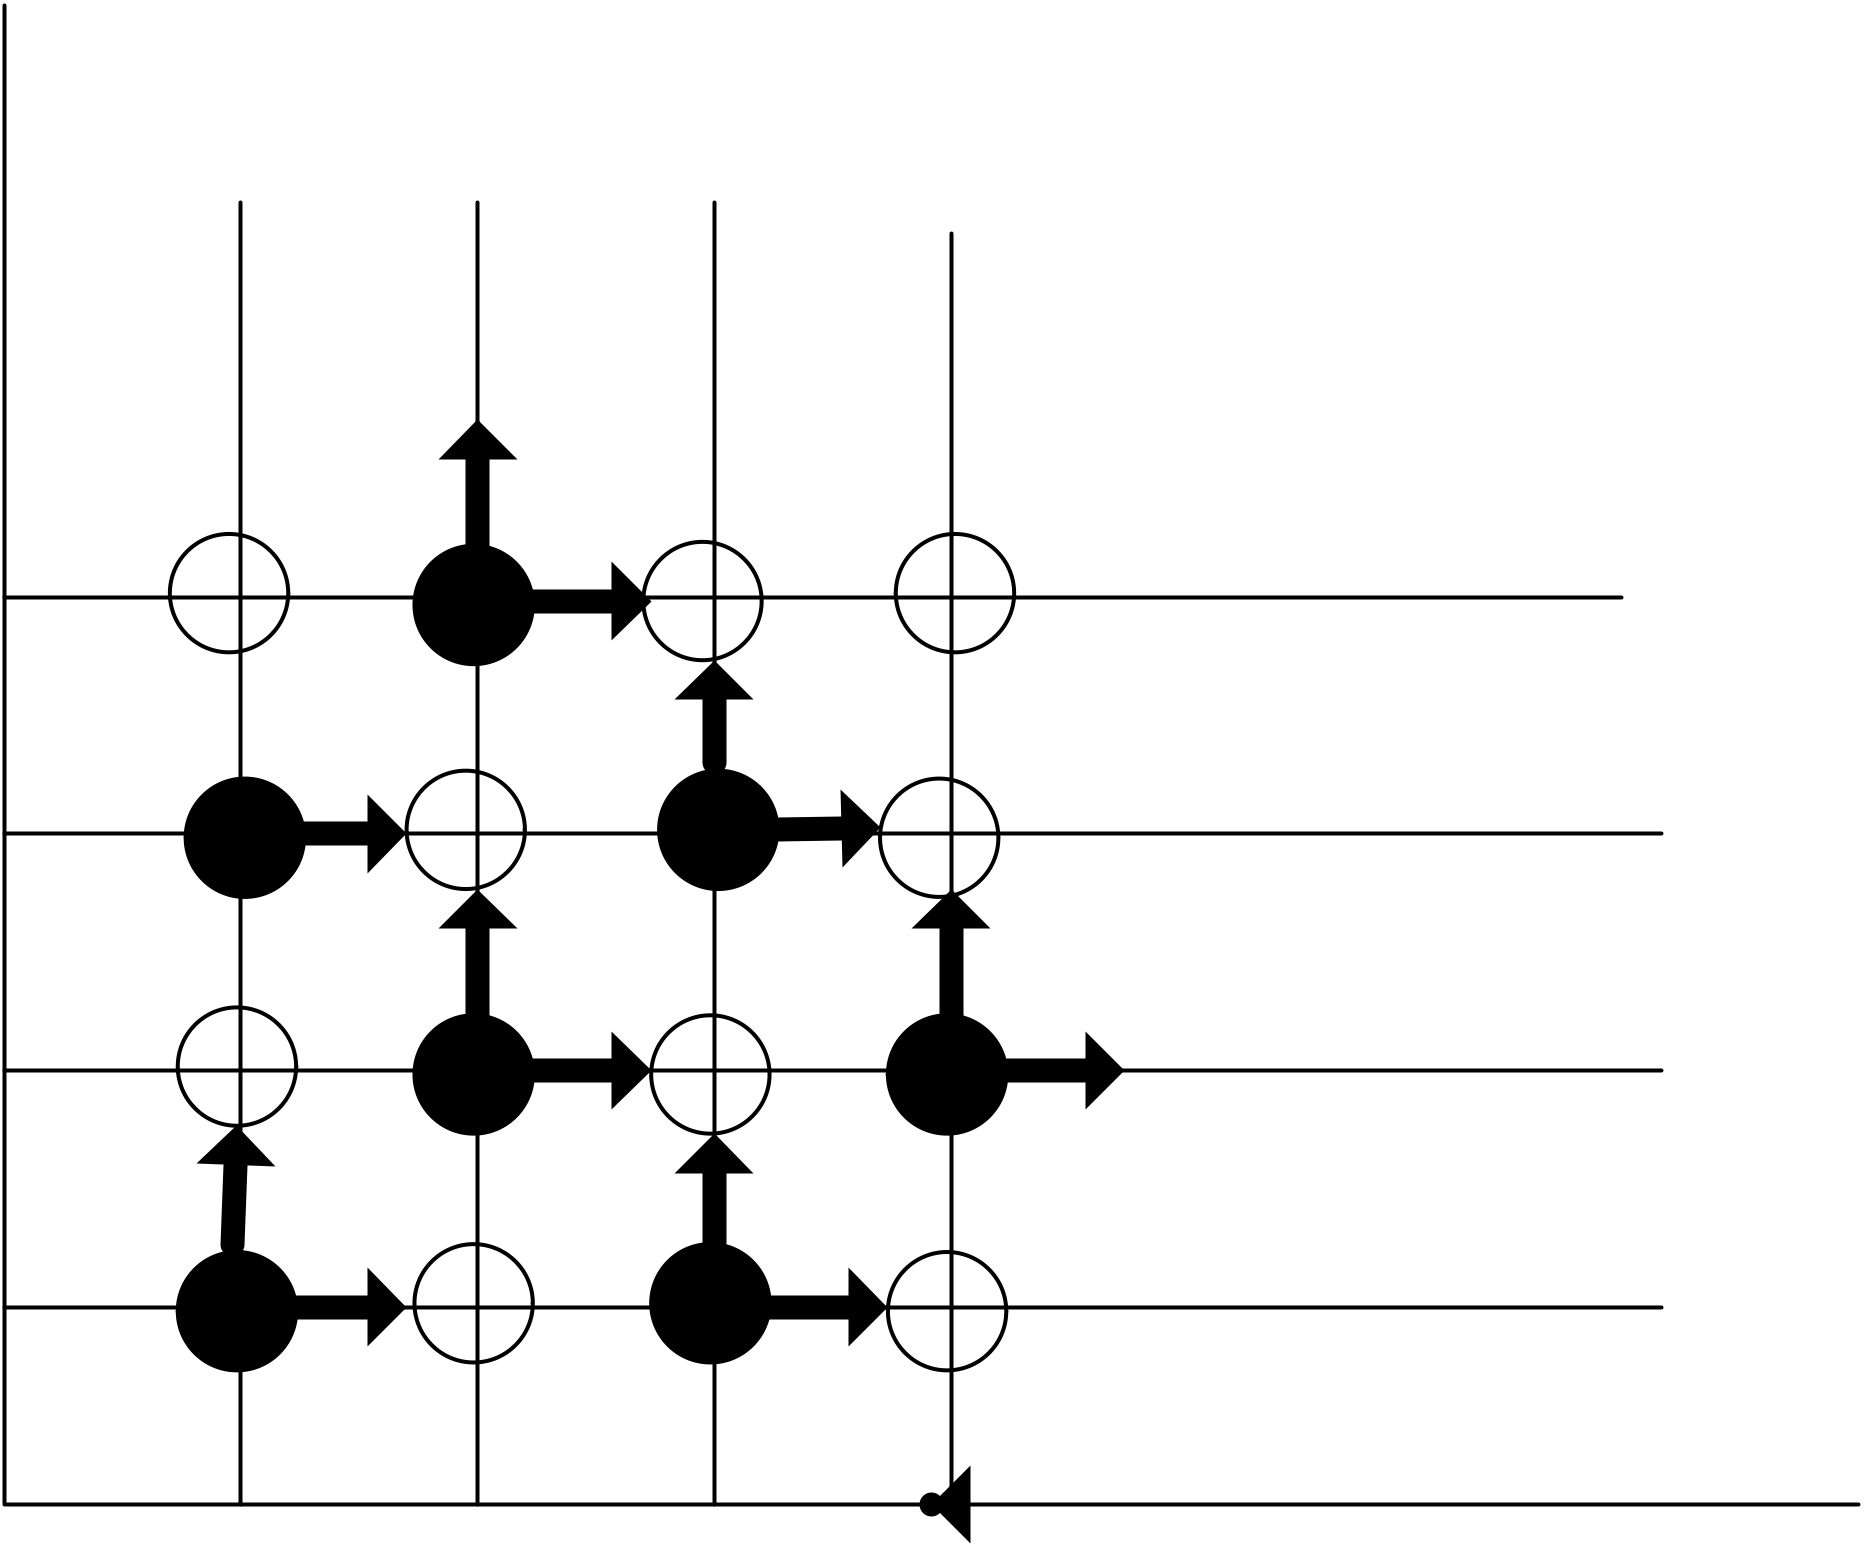
\includegraphics[scale=.1]{wavefront3c}
\end{frame}

\begin{frame}{Conclusion}
  \begin{enumerate}
  \item Wavefronts have sequential length $2n$,\\
    average parallelism~$n/2$
  \item Equivalency of wavefronts and multicolouring
  \end{enumerate}
\end{frame}

\begin{frame}{Recursive doubling}
  Write recurrence $x_i=b_i-a_{i-1}x_{i-1}$
  as
\[ 
  \begin{pmatrix}
    1&&\emptyset\\ a_{21}&1\\ &\ddots&\ddots\\ 
    \emptyset&&a_{n,n-1}&1
  \end{pmatrix}
  \begin{pmatrix}
    x_1\\ x_2\\ \vdots \\ x_n
  \end{pmatrix}
  =
  \begin{pmatrix}
    b_1\\ b_2\\ \vdots \\ b_n
  \end{pmatrix}
\]
for short: $A=I+B$
\end{frame}

\begin{frame}
Transform
\tiny
\[
  \begin{pmatrix}
    1&&&&&&&\emptyset\\ 0&1\\ &-a_{32}&1\\ &&0&1\\
    &&&-a_{54}&1\\ &&&&0&1\\ &&&&&-a_{76}&1\\ &&&&&&\ddots&\ddots\\
  \end{pmatrix}\times (I+B) =
\] \[
  \begin{pmatrix}
    1&&&&&&&\emptyset\\ a_{21}&1\\ -a_{32}a_{21}&0&1\\ 
    &&a_{43}&1\\ &&-a_{54}a_{43}&0&1\\
    &&&&a_{65}&1\\ &&&&-a_{76}a_{65}&0&1\\ &&&&&\ddots&\ddots&\ddots
  \end{pmatrix}
\]
\begin{itemize}
\item Recurrence over half the elements
\item Parallel calculation of other half
\item Now recurse\ldots
\end{itemize}
\end{frame}

\frame{\frametitle{Turning implicit operations into explicit}
Normalize ILU solve to $(I-L)$ and $(I-U)$

Approximate $(I-L)x = y$ by $x\approx (I+L+L^2)y$

Convergence guaranteed for diagonally dominant
}

